\begin{question}
\SetQuestionProperties{source = {Ex. 1,2; MW, III.17.1}}
The function $g$ takes values on the rectangles as indicated in the figure below. Calculate the integral of $g$.

\begin{center}
\begin{tabu} to \linewidth {*2{X[1,c]}}
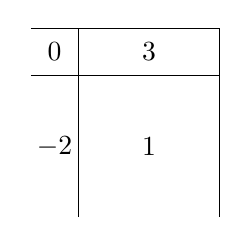
\begin{tikzpicture}[scale=0.6, baseline=0]
  \def\scale{0.6}
  % \draw[coordinate grid, step=1.] (0,0) grid (4,4);

  \drawxlabels{1/1, 4/4}
  \drawylabels{3/3, 4/4}
  \drawaxes{0}{0}{4.4}{4.4}

  \draw (1,0) -- (1,4);
  \draw (4,0) -- (4,4);
  \draw (0,3) -- (4,3);
  \draw (0,4) -- (4,4);

  \node at (0.5, 1.5) {$-2$};
  \node at (0.5, 3.5) {$0$};
  \node at (2.5, 1.5) {$1$};
  \node at (2.5, 3.5) {$3$};
\end{tikzpicture}
&
%0.9375
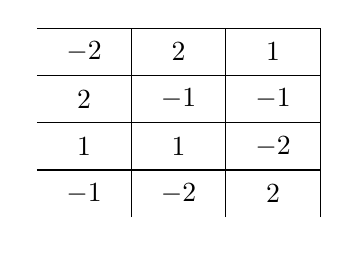
\begin{tikzpicture}[scale=0.6, baseline=(X.base)]
  \def\scale{0.6}
  \node at (0,0) (X) {};

  \drawaxes{0}{0}{6.6}{4.4}

  \foreach \x in {2, 4, 6} {
    \draw (\x, 0) -- (\x, 4);
  }

  \foreach \y in {1, 2, 3, 4} {
    \draw (0, \y) -- (6, \y);
  }

  \foreach \x/\y/\text in {1/0.5/-1, 1/1.5/1, 1/2.5/2, 1/3.5/-2,
                           3/0.5/-2, 3/1.5/1, 3/2.5/-1, 3/3.5/2,
                           5/0.5/2, 5/1.5/-2, 5/2.5/-1, 5/3.5/1} {
    \node at (\x, \y) {$\text$};
  }

  \drawxlabels{2/2, 4/4, 6/6};
  \drawylabels{1/1, 2/2, 3/3, 4/4};
\end{tikzpicture}
\\
(a) & (b)
\end{tabu}
\end{center}
\end{question}

\begin{solution}
\begin{enumerate}
\item
Denote the rectangle $D = [0,4] \x [0,4]$. Because $g$ is a step function, we can evaluate the integral as follows
\[
\iint_D g(x,y) \ud x \ud y =
-2 \cdot 3 + 1 \cdot 9 + 0 \cdot 1 + 3 \cdot 3 = 12\,.
\]
\item
Similarly to the previous exercise, let $D = [0,6] \x [0,4]$. Each smaller rectangle has the same area $2$ and therefore
\begin{align*}
\iint_D g(x,y) \ud x \ud y &=
-2 \cdot \left( -2 + 2 + 1 + 2 -1 -1 + 1 + 1 -2 -1 -2 + 2\right)
= 0\,.
\end{align*}
\end{enumerate}
\end{solution}

\begin{question}
\SetQuestionProperties{source = {Ex. 5; MW, III.17.1}}
Evaluate the iterated integrals
\begin{tasks}(2)
\task
$\displaystyle \int_0^3 \int_0^2 x^3 y \ud x \ud y$.
\task
$\displaystyle \int_0^3 \int_0^2 x^3 y \ud y \ud x$.
\end{tasks}
\end{question}

\begin{solution}
\begin{enumerate}
\item
We have
\begin{align*}
\int_0^3 \int_0^2 x^3 y \ud x \ud y
&= \int_0^3 \frac 14 x^4 y \bigg|_{x=0}^2 \ud y
= 4 \int_0^3 y \ud y = 18\,.
\end{align*}

\item
We have
\begin{align*}
\int_0^3 \int_0^2 x^3 y \ud y \ud x
&= \int_0^3 \frac 12 x^3 y^2 \bigg|_{y=0}^2 \ud x
= \int_0^3 2 x^3 \ud x = \frac{81}{2} \,.
\end{align*}
\end{enumerate}
\end{solution}

\begin{question}
\SetQuestionProperties{source = {Ex. 12, 14--16; MW, III.17.1}}
Evaluate $\displaystyle\iint_{D} f(x,y) \ud x \ud y$ for the following functions and rectangles.
\begin{tasks}(2)
\task
$f(x,y) = xy^3 e^{x^2 y^2}$; $D=[1,3] \x [1,2]$.
\task
$\displaystyle f(x,y) = xy + \frac{x}{y+1}$; $D=[1,4]\x [1,2]$.
\task
$\displaystyle f(x,y) = y^3 \cos^2 x$; $D=[-1,2]\x [0,2]$.

{\itshape Hint:} Use half-angle formulas for $\cos^2 x$.
\task
$\displaystyle f(x,y) = y^5 \sin x\, e^{y^3 \cos x}$; $D=[0,1]\x [-1,0]$.
\end{tasks}
\end{question}

\begin{solution}
\begin{enumerate}
\item
We have
\begin{align*}
\int_1^2 \int_1^3 xy^4 e^{x^2y^2} \ud x \ud y
&= \int_1^2 \frac 12 y e^{x^2y^2} \bigg|_{x=1}^3 \ud y
= \int_1^2 \frac 12 y \left( e^{9y^2} - e^{y^2}\right) \ud y \\
&= \frac{1}{36} e^{9y^2} - \frac{1}{4} e^{y^2} \bigg|_{y=1}^2
= \frac{1}{36} \left(e^{36} - e^9\right) - \frac{1}{4} \left(e^4 - e\right)\,.
\end{align*}
\item We have
\begin{align*}
\int_1^4 \int_1^2 xy + \frac{x}{y+1} \ud y \ud x
&= \int_1^4 x \ud x \int_1^2 y + \frac{1}{y+1} \ud y \\
&= \left(\left. \frac{x^2}2 \right|_{x=1}^4 \right) \left(\left. \frac{y^2}2 + \ln(y+1) \right|_{y=1}^2 \right)
= \frac {45}4 + \frac{15}2 \ln \frac 32\,.
\end{align*}
\item
We have
\begin{align*}
\int_{-1}^2 \int_0^2 y^3 \cos^2 x \ud y \ud x &=
\int_{-1}^2 \frac 14 y^4 \cos^2 x \bigg|_{y=0}^2 \ud x
= \int_{-1}^2 4 \cos^2 x \ud x 
= \int_{-1}^2 2 + 2\cos 2x \ud x \\
&= 2x + \sin 2x \bigg|_{x={-1}}^2 = 6 + \sin 2 + \sin 4\,.
\end{align*}
\item
We choose the following order of integration
\begin{align*}
\int_{-1}^0 \int_0^1 y^5 \sin x\, e^{y^3 \cos x} \ud x \ud y
&= \int_{-1}^0 -y^2 e^{y^3 \cos x} \bigg|_{x=0}^1 \ud y
= \int_{-1}^0 -y^2 e^{y^3 \cos 1} + y^2 e^{y^3}\ud y \\
&= \left.\frac{-1}{3\cos 1} e^{y^3 \cos 1} + \frac 13 e^{y^3} \right|_{y=-1}^0 \\
&= \frac 13 - \frac 1{3e} + \frac{1}{3\cos 1}\left(e^{-\cos 1} - 1\right)\,.
\end{align*}
\end{enumerate}
\end{solution}

\begin{question}
\SetQuestionProperties{source = {Ex. 19; MW, III.17.1}}
Find the volume under the graph of
\[
f(x,y) = x^3 + y^2 + 2\,,
\]
between the planes
\[
x=-1, x=1, y=1 \text{ and } y=3\,.
\]
\end{question}

\begin{solution}
The volume is given by the integral
\begin{align*}
\iint_{[-1,1]\times [1,3]} x^3 + y^2 + 2 \ud x \ud y
&= \int_{-1}^1 \int_1^3 x^3 + y^2 + 2 \ud y \ud x \\
&= \int_{-1}^1 x^3y + \frac 13 y^3 + 2y \bigg|_{y=1}^3 \ud x
= \int_{-1}^1 2x^3 + \frac{38}3 \ud x \\
&= \frac 12 x^4 + \frac{38}3x \bigg|_{x=-1}^1 = \frac{76}{3}\,.
\end{align*}
\end{solution}

\begin{question}
\SetQuestionProperties{source = {Ex. 21; MW, III.17.1}}
The density at each point of a $1$ centimeter square (i.e., each side has length $1$ centimeter) microchip is $4+r^2$ grams per square centimeter, where $r$ is the distance in centimeters from the point to the center of the chip. What is the mass of the chip?
\end{question}

\begin{solution}
We model the chip as the rectangle $D = \left[-\frac 12, \frac 12\right] \x \left[-\frac 12, \frac 12\right]$. Then the center is the point $(0,0)$ and the squared distance of a point $(x,y)$ to the center is $r^2 = x^2 + y^2$. Thus the mass $m$ can be computed as
\begin{align*}
m &= \int_{-1/2}^{1/2} \int_{-1/2}^{1/2} 4 + x^2 + y^2 \ud x \ud y
= \int_{-1/2}^{1/2} 4x + \frac 13 x^3 + xy^2 \bigg|_{x={-1/2}^{1/2}} \ud y
= \int_{-1/2}^{1/2} 4 + \frac 1{12} + y^2 \ud y \\
&= 4y + \frac 1{12}y + \frac 13 y^3 \bigg|_{y=-1/2}^{1/2}
= 4 + \frac 1{12} + \frac{1}{12} = \frac{25}{6}\,.
\end{align*}
\end{solution}

\begin{question}
\SetQuestionProperties{difficulty={*}}
Using the fact that for $x,y > 0$,
\[
\frac{\p^2}{\p x \p y} \arctan \frac xy = \frac{x^2-y^2}{\left(x^2 + y^2 \right)^2}\,,
\]
show that
\begin{align*}
\int_0^1 \left( \int_0^1 \frac{x^2-y^2}{\left(x^2 + y^2 \right)^2} \ud y \right) \ud x
&= \frac \pi 4 &
\int_0^1 \left( \int_0^1 \frac{x^2-y^2}{\left(x^2 + y^2 \right)^2} \ud x \right) \ud y
&= -\frac \pi 4\,.
\end{align*}

\begin{note*}
This problem shows that the order of integration sometimes does matter. The problem here is that the function $\frac{x^2-y^2}{\left(x^2 + y^2 \right)^2}$ is not integrable over the rectangle $R = [0,1] \x [0,1]$, which means that we cannot apply the theorem, that reduces the double integral to an iterated integral; the double integral $\iint_R \frac{x^2-y^2}{\left(x^2 + y^2 \right)^2} \ud x \ud y$ does not exist. This example was found already by Cauchy in 1814\footfullcite[p.178]{Elstrodt2011}.
\end{note*}
\end{question}

%%% Local Variables:
%%% TeX-master: "problems"
%%% End:
